% Copyright 2018-2022 FIUS
%
% This file is part of theo-vorkurs-folien.
%
% theo-vorkurs-folien is free software: you can redistribute it and/or modify
% it under the terms of the GNU General Public License as published by
% the Free Software Foundation, either version 3 of the License, or
% (at your option) any later version.
%
% theo-vorkurs-folien is distributed in the hope that it will be useful,
% but WITHOUT ANY WARRANTY; without even the implied warranty of
% MERCHANTABILITY or FITNESS FOR A PARTICULAR PURPOSE.  See the
% GNU General Public License for more details.
%
% You should have received a copy of the GNU General Public License
% along with theo-vorkurs-folien.  If not, see <https://www.gnu.org/licenses/>.

\subsubsection{formale Notation}
\begin{frame}[fragile]{Formale Notation}
    Wir beschreiben eine \alert{\emph{Grammatik}} durch ein geordnetes \alert{\emph{Tupel}} $G = (V, \Sigma, P, S)$
    \begin{itemize}
        \item $V$ ist die Menge der verwendeten Nichtterminale
        \item $\Sigma$ die Menge der Terminale bzw. unser Alphabet
        \item $P$ ist die Menge der Produktionsregeln
        \item $S$ ist die Startvariable
    \end{itemize}
    \metroset{block=fill}
    \begin{exampleblock}{Beispiel für  L = \{$ww^R \mid w \in \{a, b\}^n, \; n \geq 1$\}}
        $G = (V,\Sigma,P,S)$ mit\\
        $V = \{S\}$\\
        $\Sigma = \{a,b\}$\\
        $P = \{S \rightarrow aSa, S \rightarrow bSb, S \rightarrow aa, S \rightarrow bb$\}\\
        \qquad bzw. kurz: $P = \{S \rightarrow aSa\ |\ bSb\ |\ aa\ |\ bb$\}
    \end{exampleblock}
\end{frame}

{\setbeamercolor{palette primary}{bg=ExColor}
\begin{frame}{Denkpause}
    \begin{columns}
        \column{0.5\textwidth}
        \begin{alertblock}{Knifflige Aufgabe}
            Bob will durch das Labyrinth laufen. Er hat folgende Möglichkeiten:\\
            $\Sigma = \{\text{\Rewind}, \text{\MoveUp}, \text{\Forward}, \text{\MoveDown}\}$
            \begin{itemize}
                \item Bob kann nicht auf ein Feld zurücktreten, von dem er gerade kam
                \item Bob geht bei jedem Schritt ein Feld in die angegebene Richtung
            \end{itemize}
        \end{alertblock}
        \column{0.5\textwidth}
        \begin{figure}
            \centering
            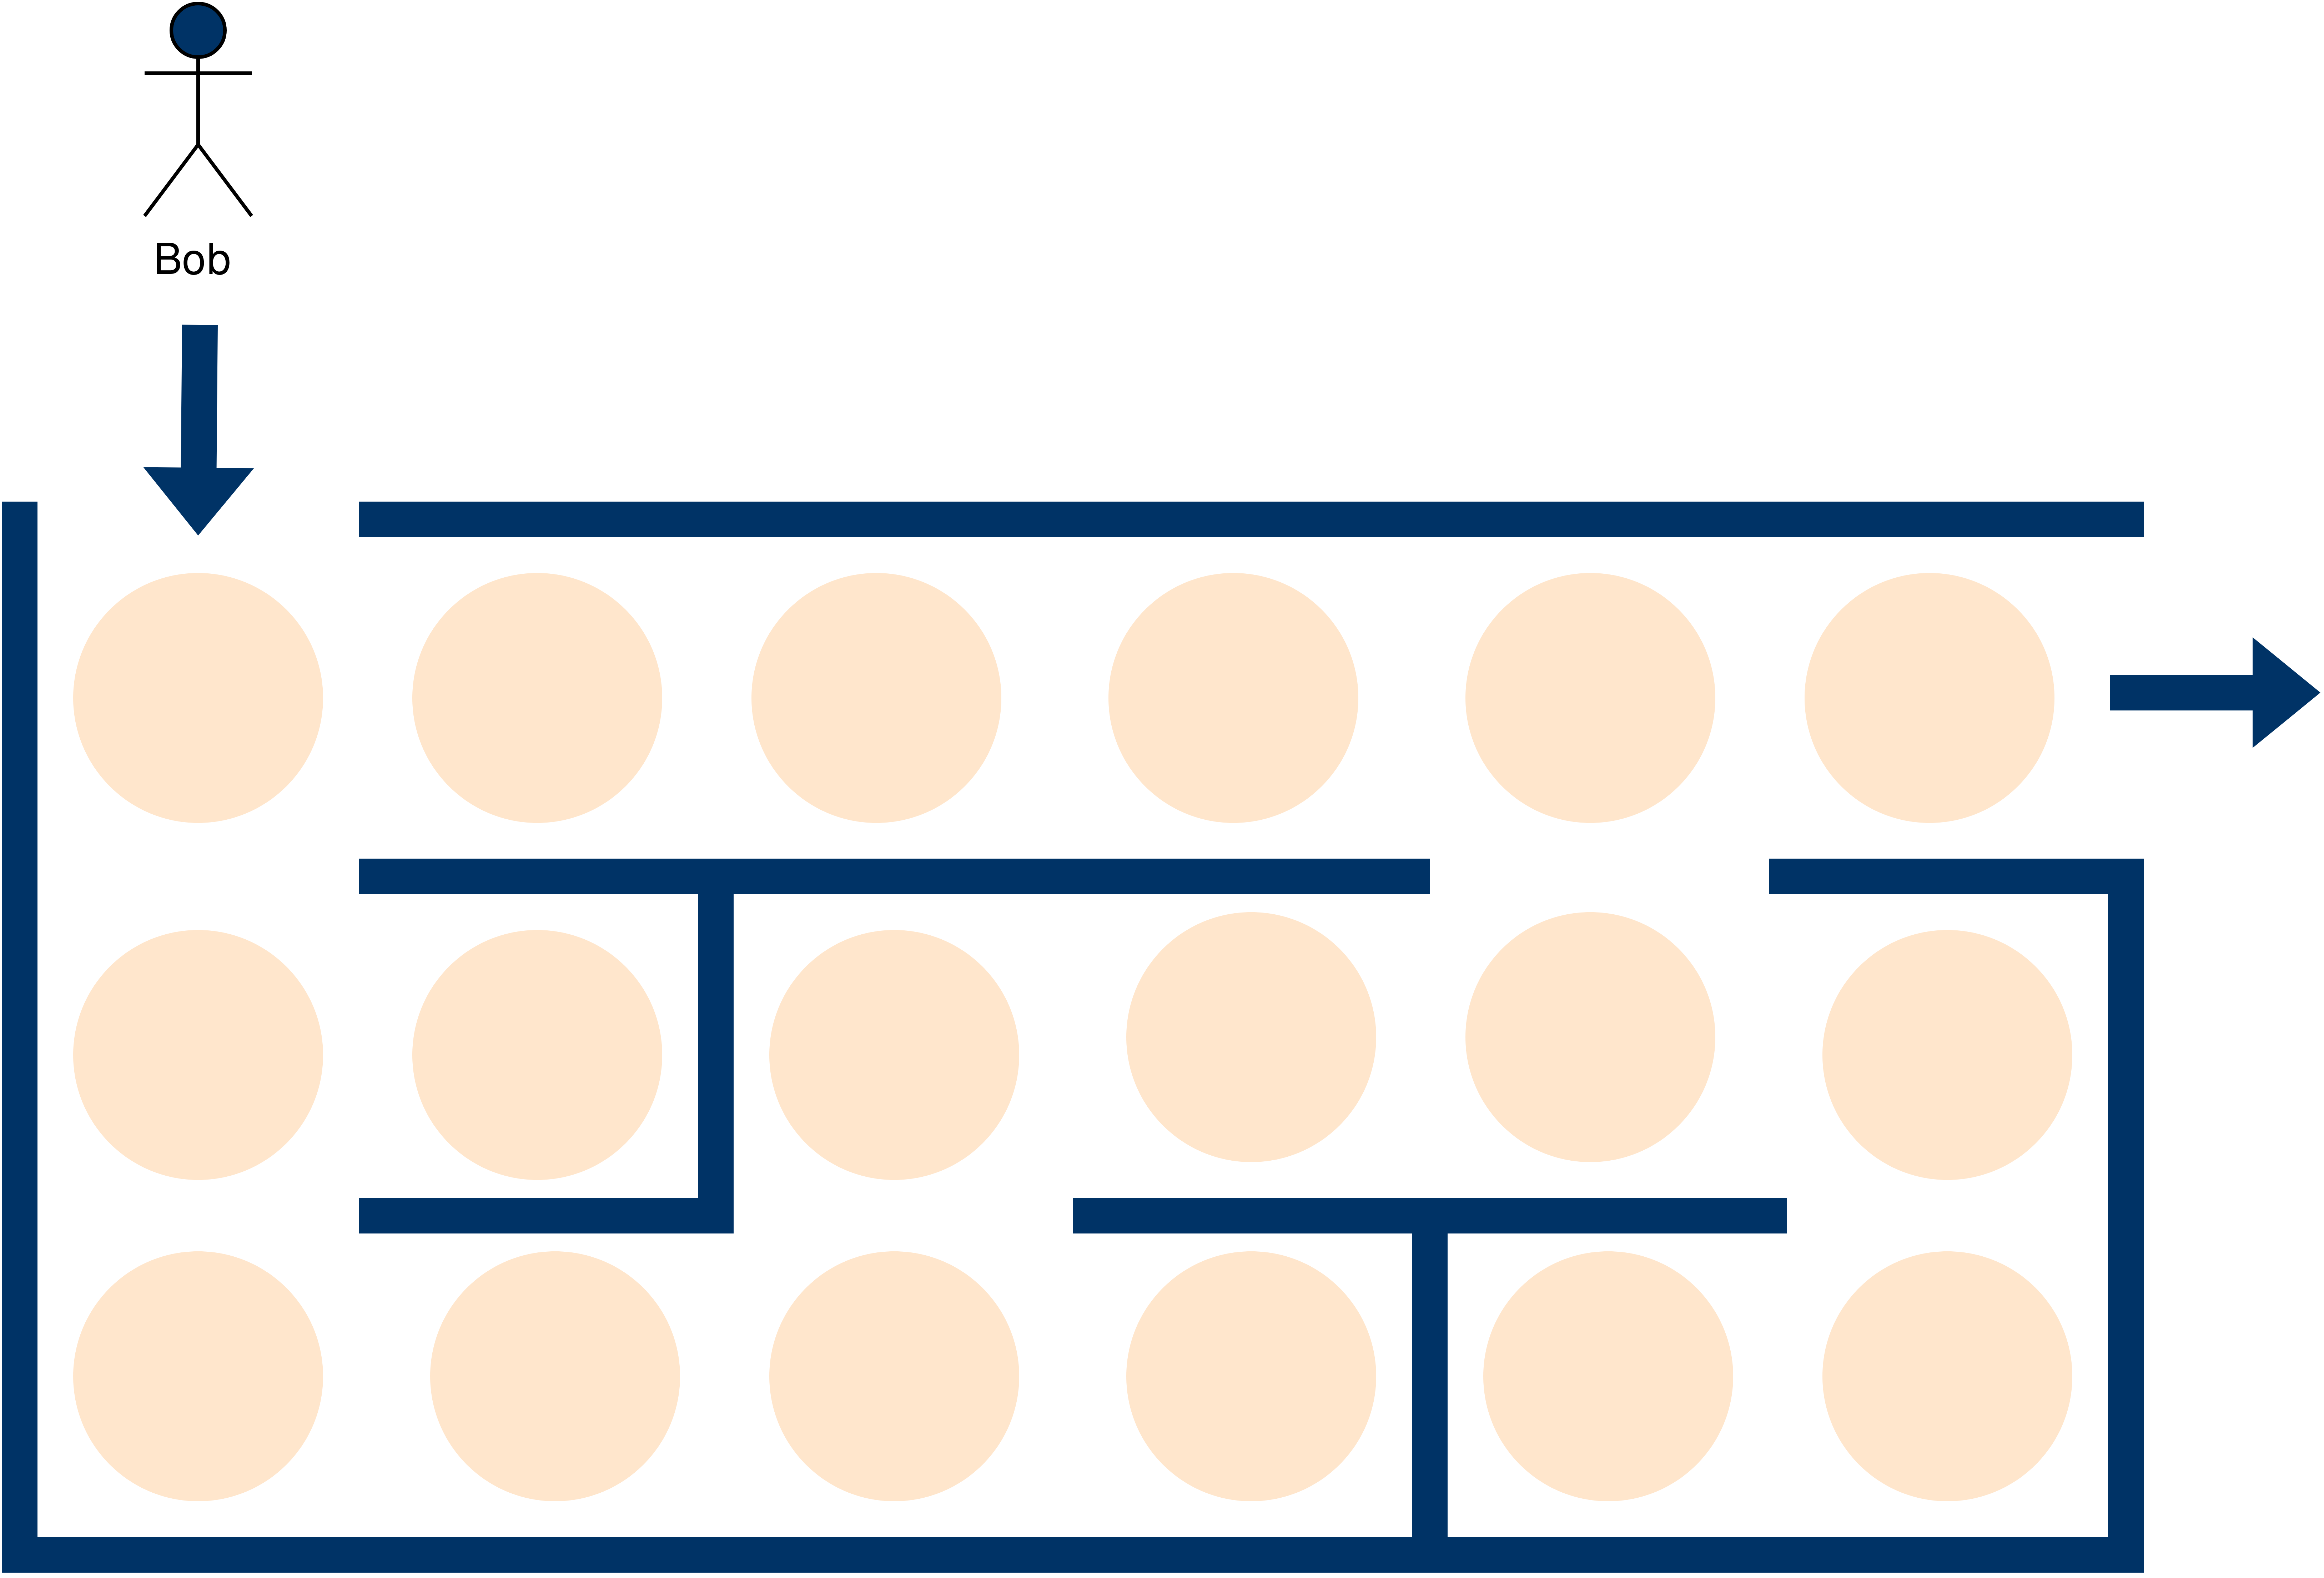
\includegraphics[width=0.7\textwidth]{../figures/GBeispiel.png}
            \caption{Bobs Problem}

        \end{figure}
    \end{columns}
    \alert{Geben Sie eine Grammatik an, welche die Sprache beschreibt, die Bob durch alle ihm möglichen Wege des Labyrinths führt.}
\end{frame}
}

{\setbeamercolor{palette primary}{bg=ExColor}
\begin{frame}{Denkpause}
    \begin{alertblock}{Beispiel}
        \begin{figure}
            \centering
            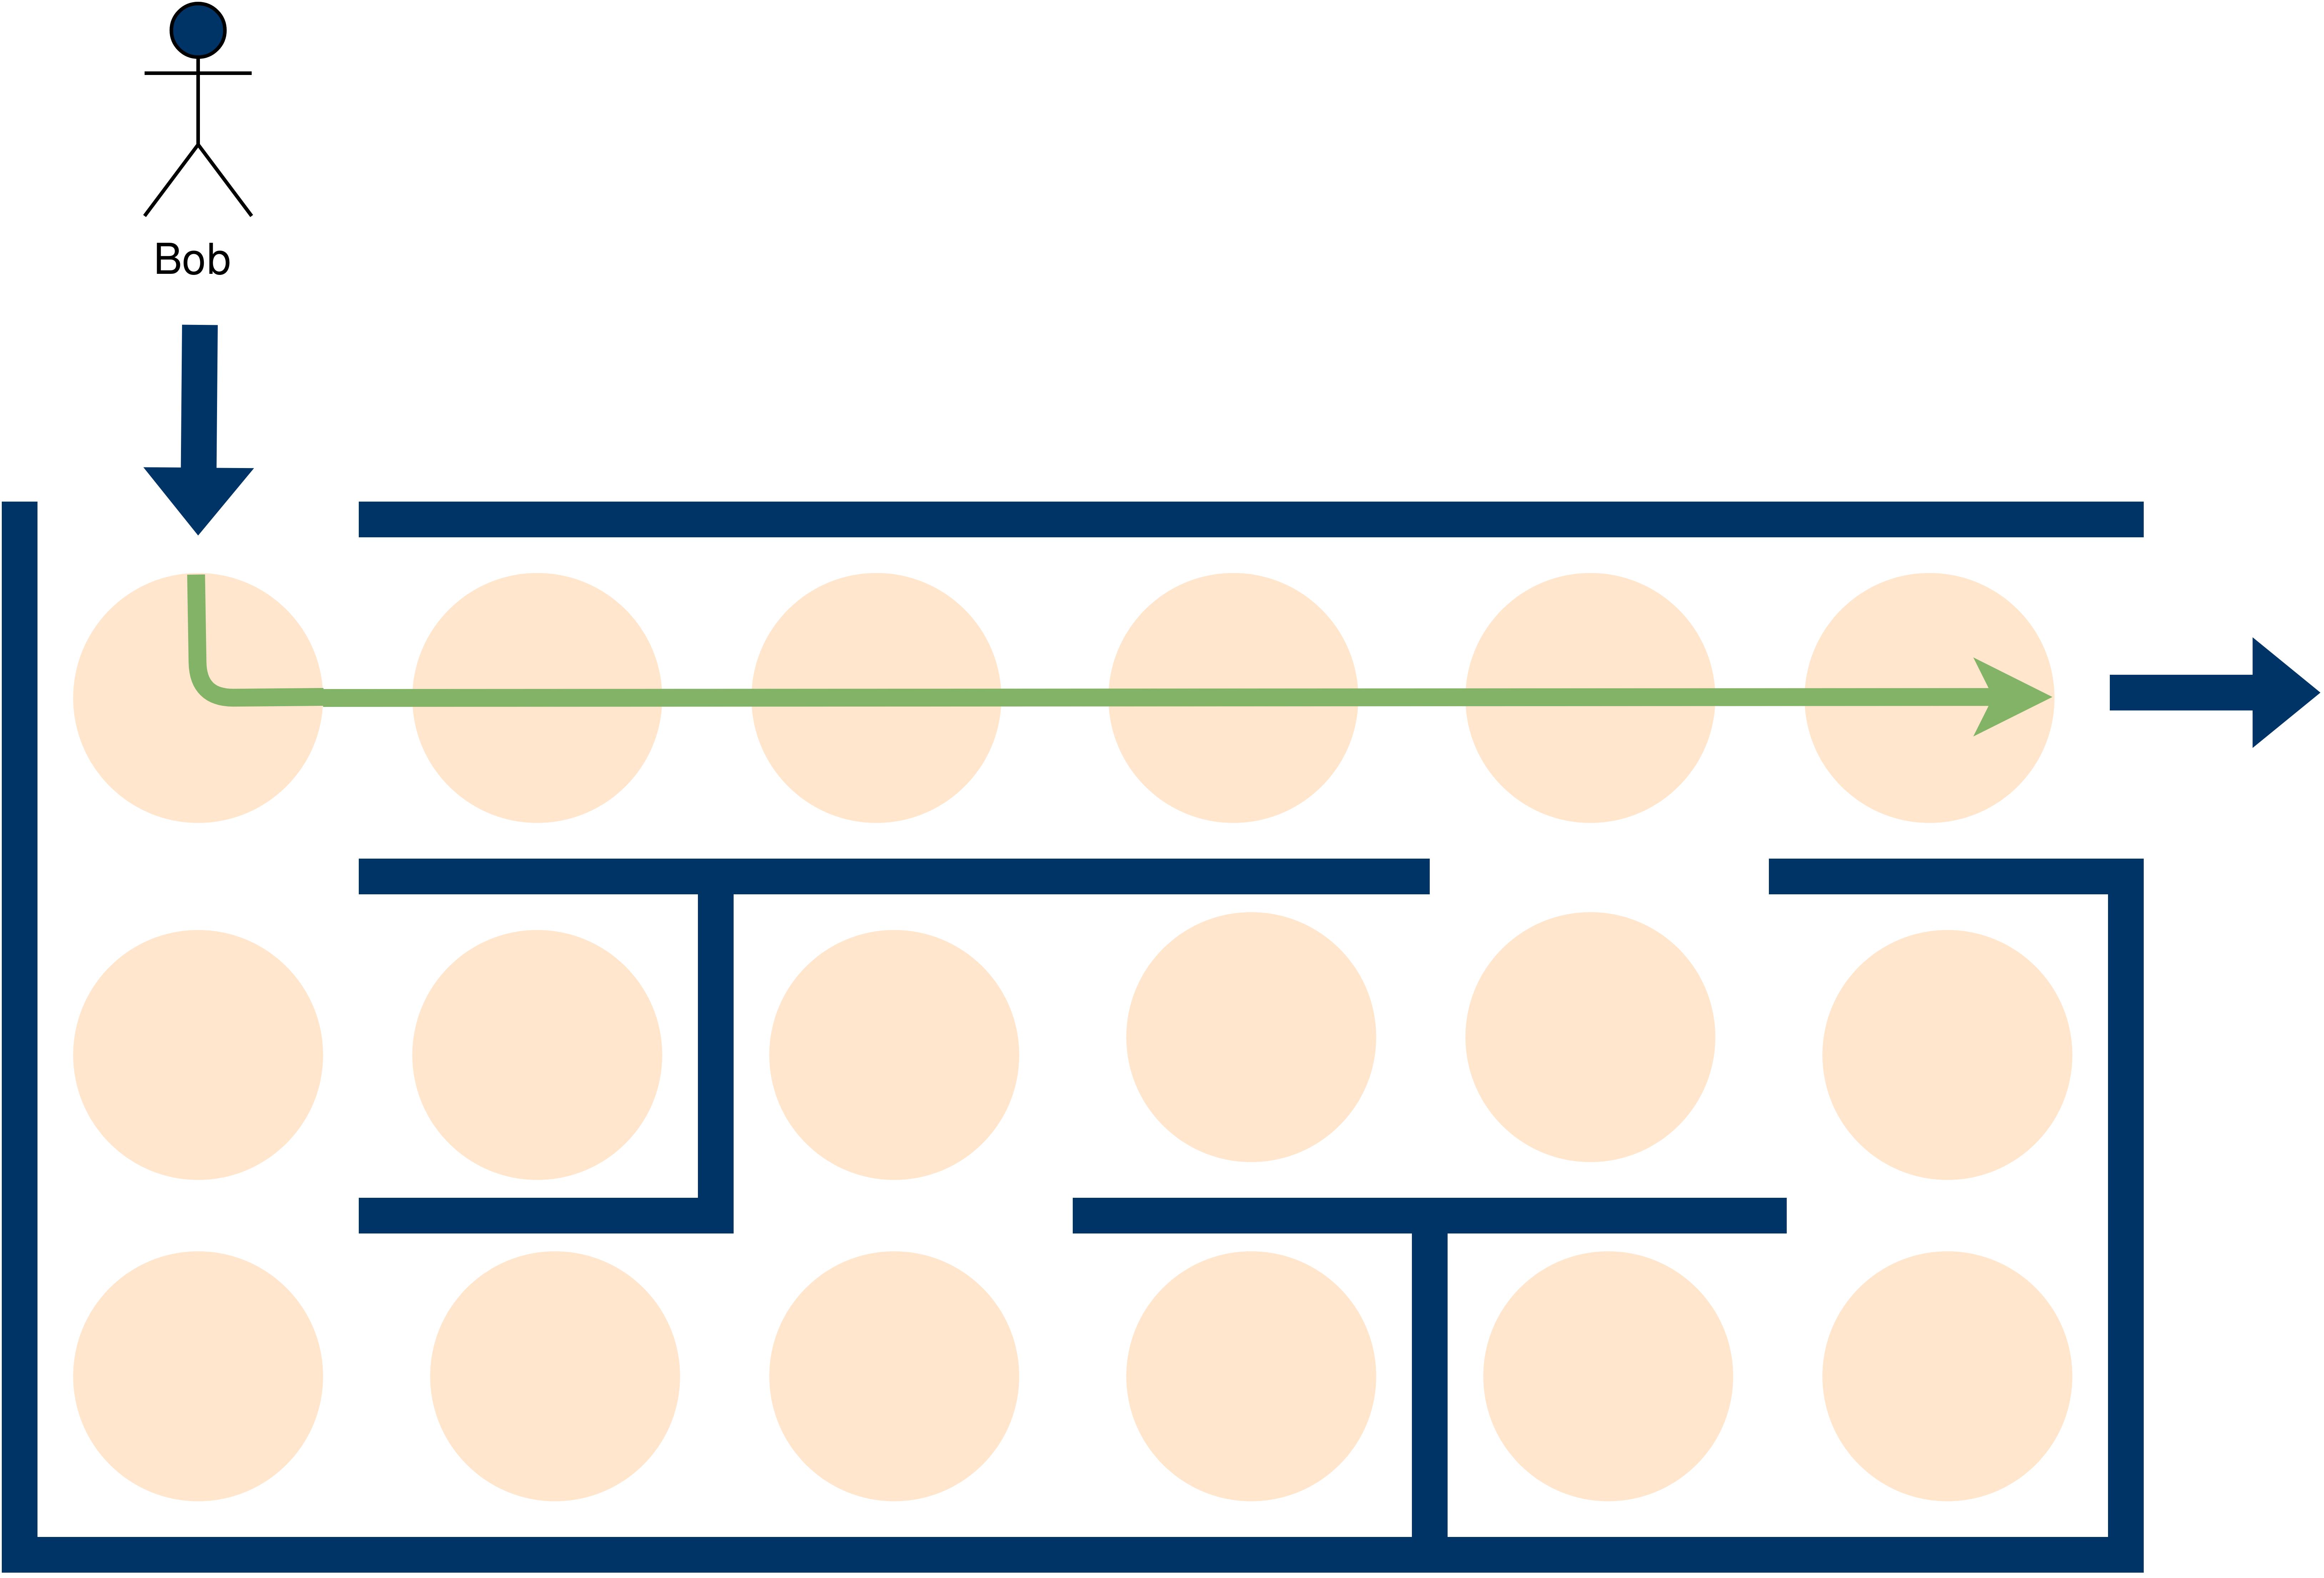
\includegraphics[width=0.7\textwidth]{../figures/GBeispiel1.png}
            \caption{Der direkte Weg ist repräsentiert durch das Wort \alert{\MoveDown\Forward\Forward\Forward\Forward\Forward\Forward}}
        \end{figure}
    \end{alertblock}
\end{frame}
}

{\setbeamercolor{palette primary}{bg=ExColor}
\begin{frame}<handout:0>{Lösung}
    \only<1>{
        \begin{figure}
            \centering
            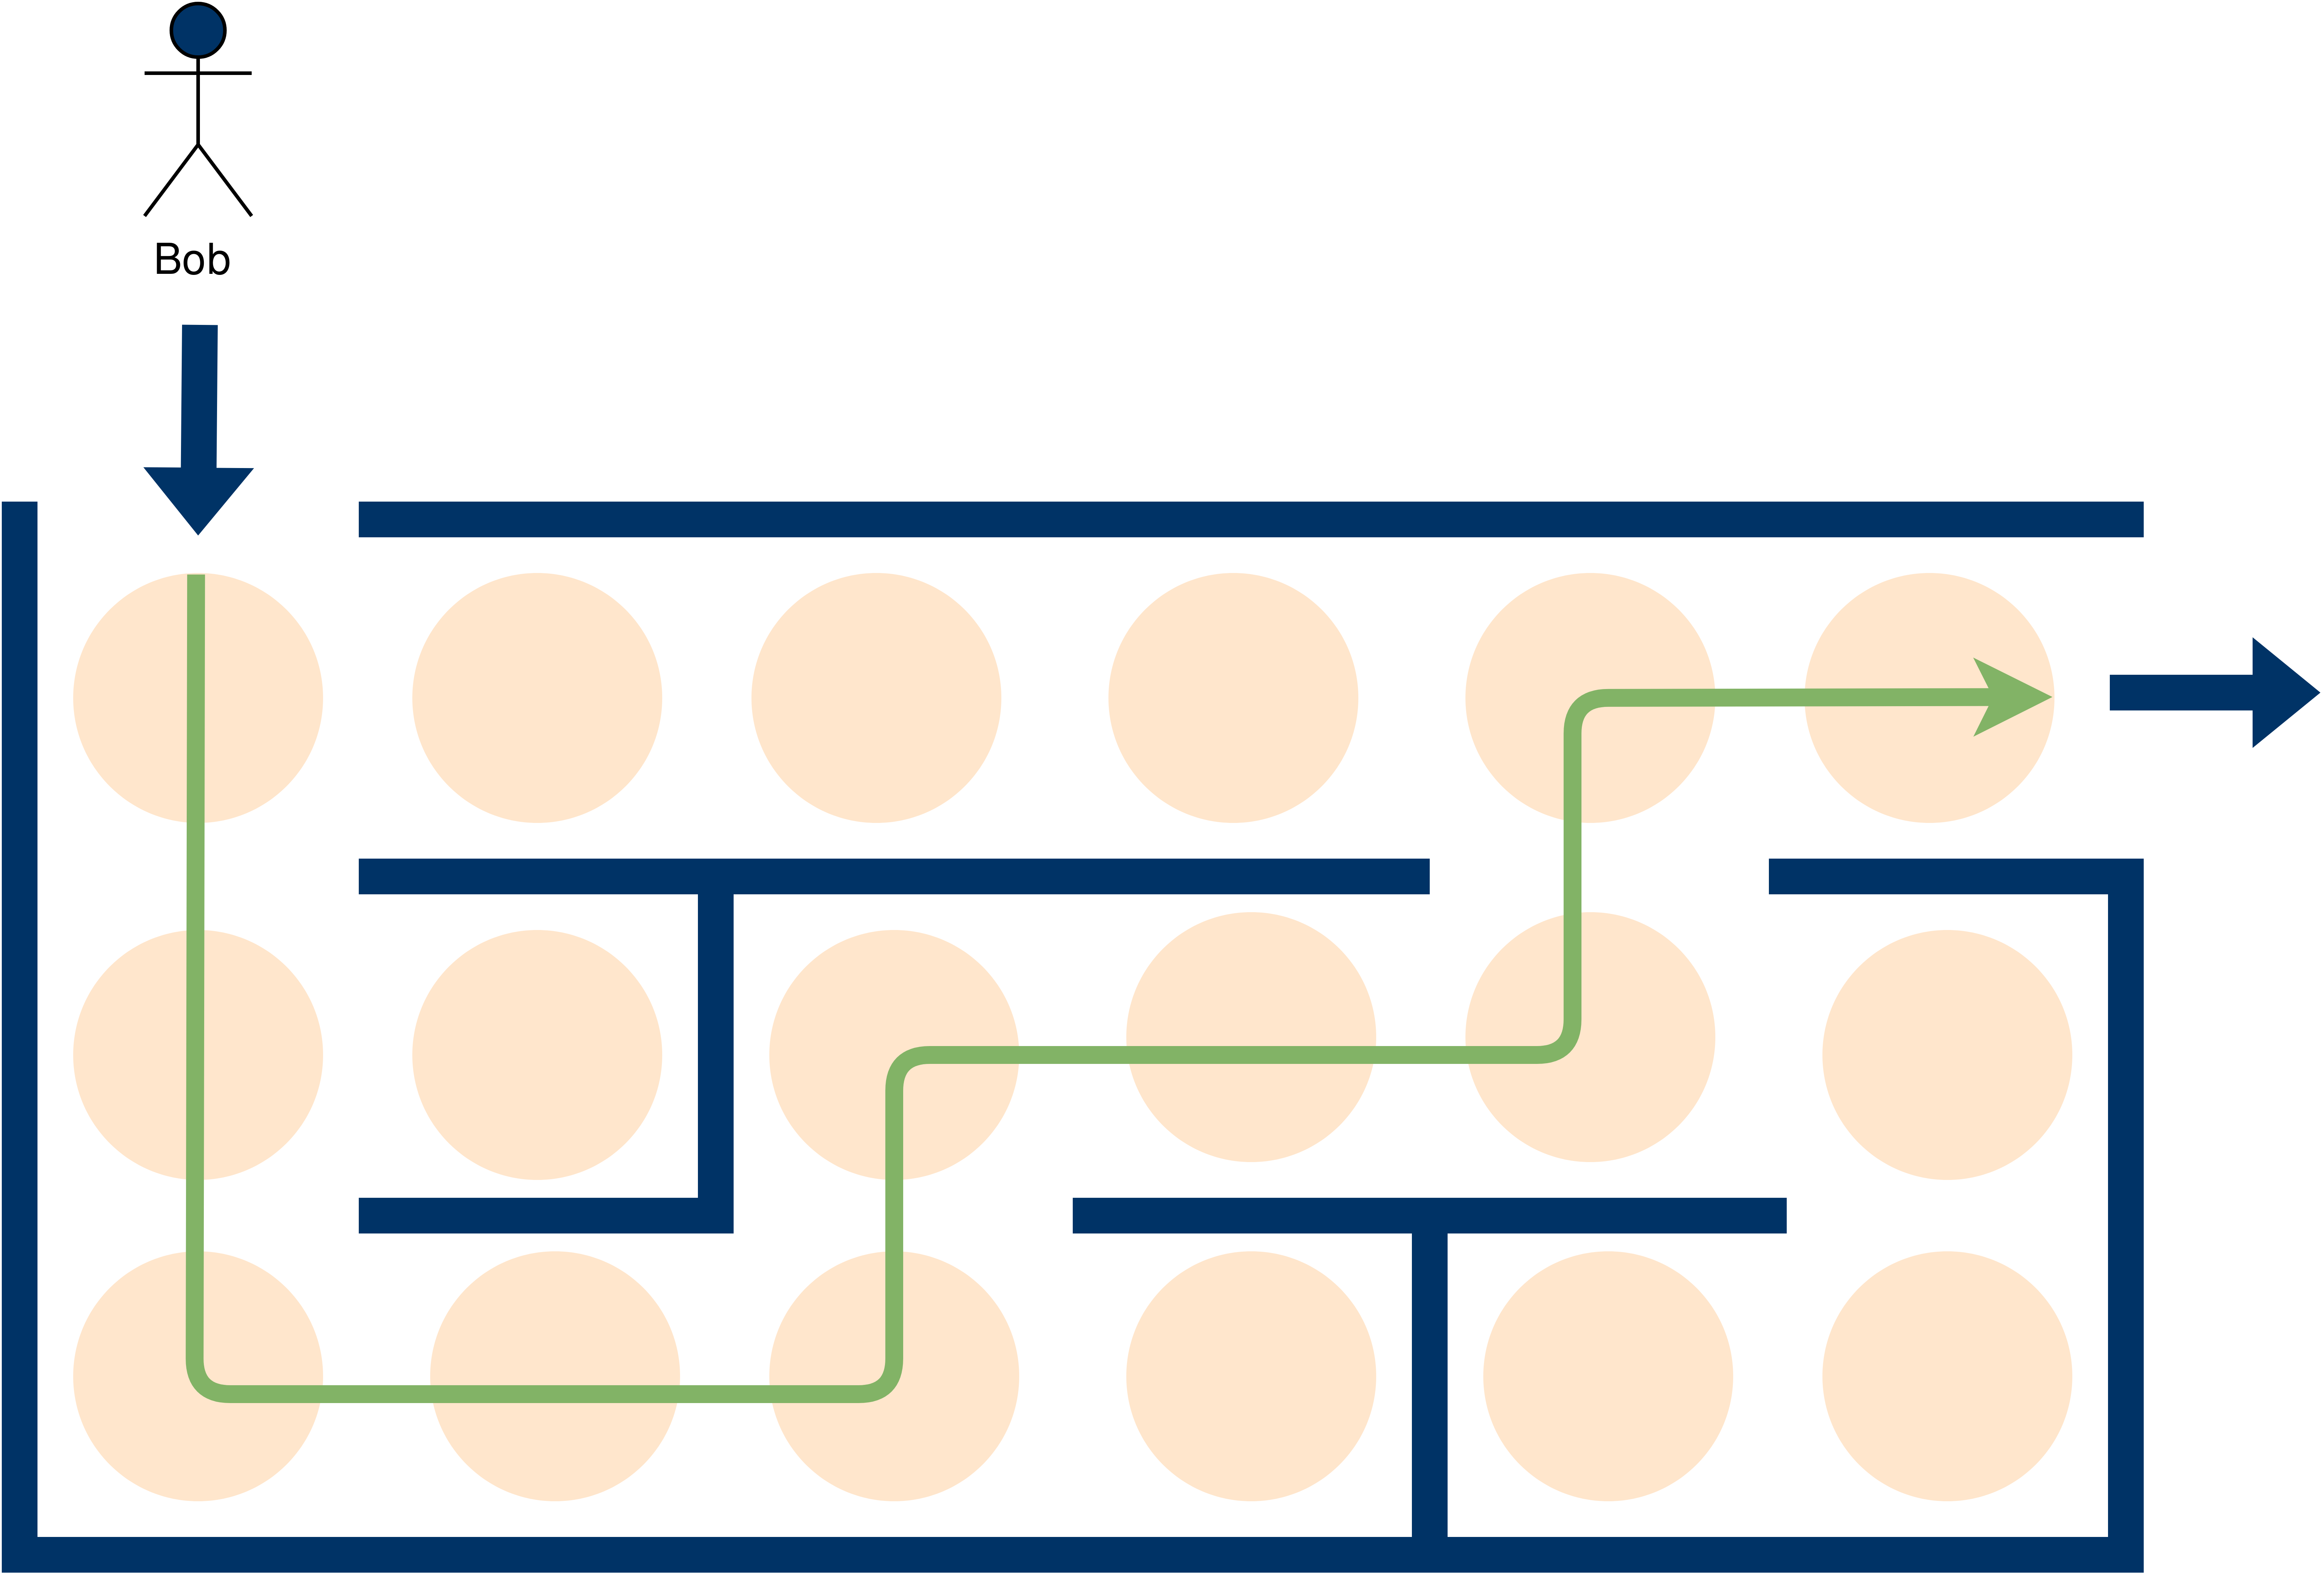
\includegraphics[width=0.7\textwidth]{../figures/GBeispiel2.png}
            \caption{Indirekter Weg}

        \end{figure}
    }
    \only<2>{
        \begin{figure}
            \centering
            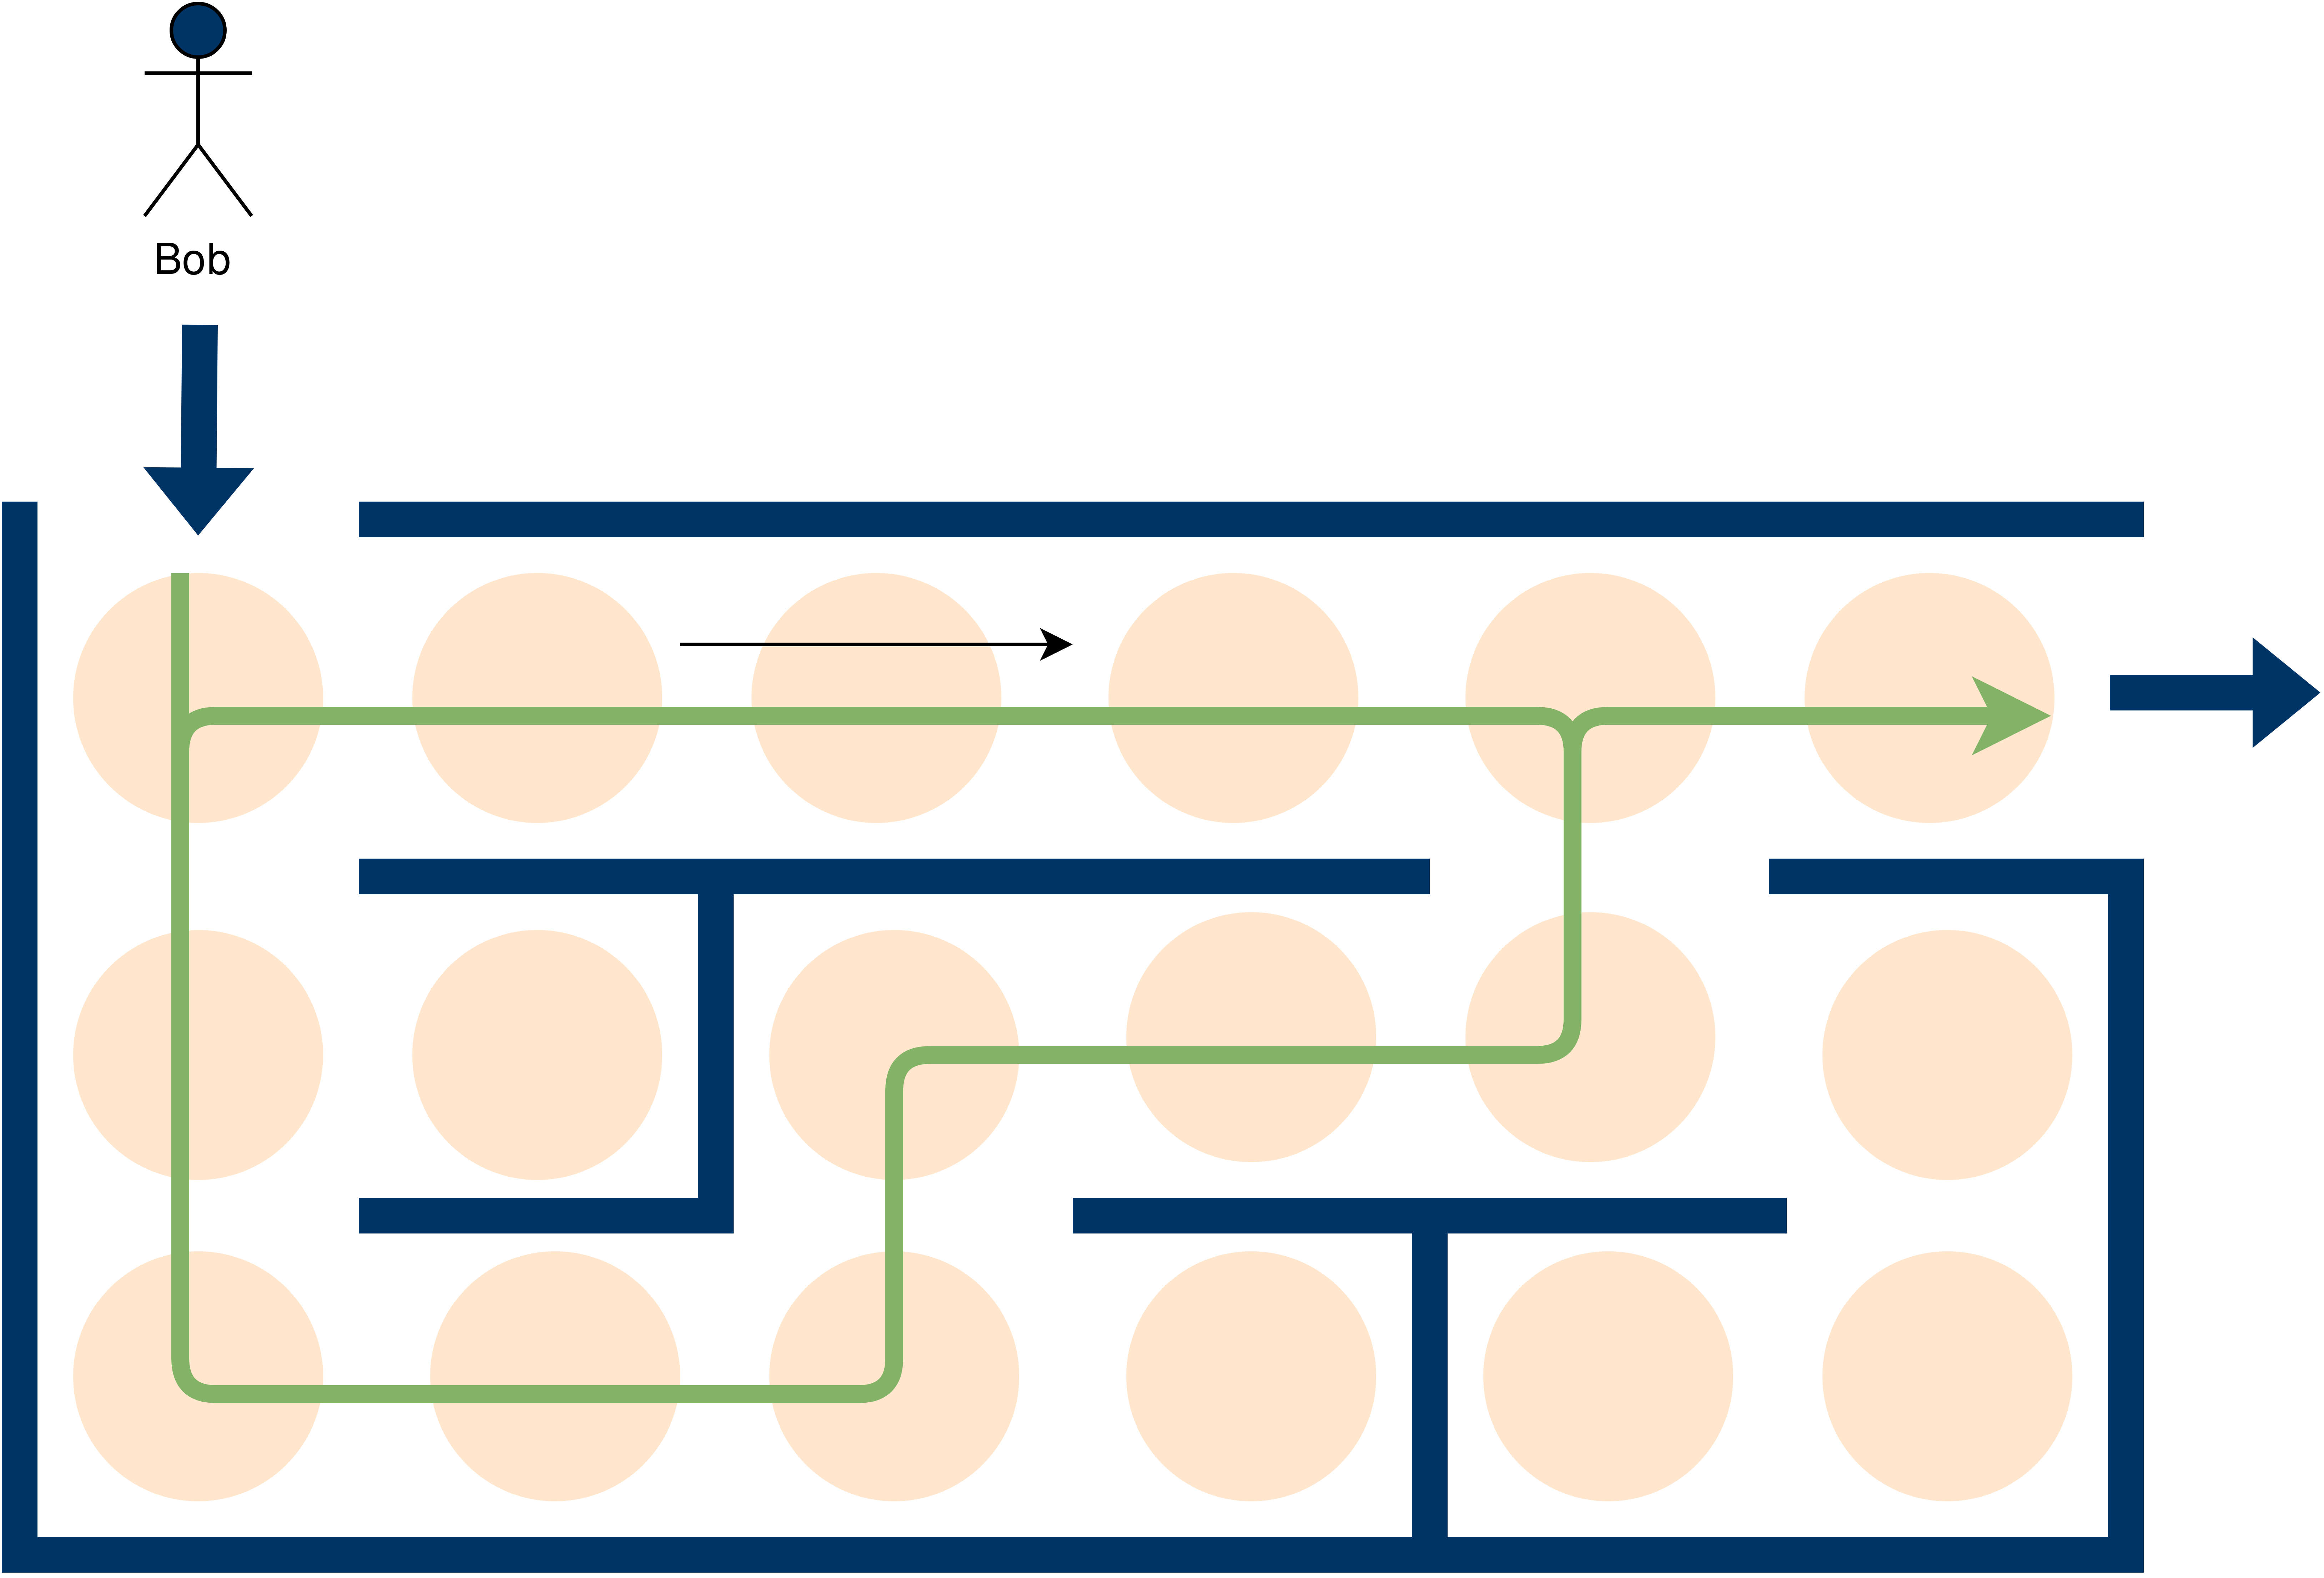
\includegraphics[width=0.7\textwidth]{../figures/GBeispiel3.png}
            \caption{Schlaufe Uhrzeigersinn}

        \end{figure}\textbf{}
    }
    \only<3>{
        \begin{figure}
            \centering
            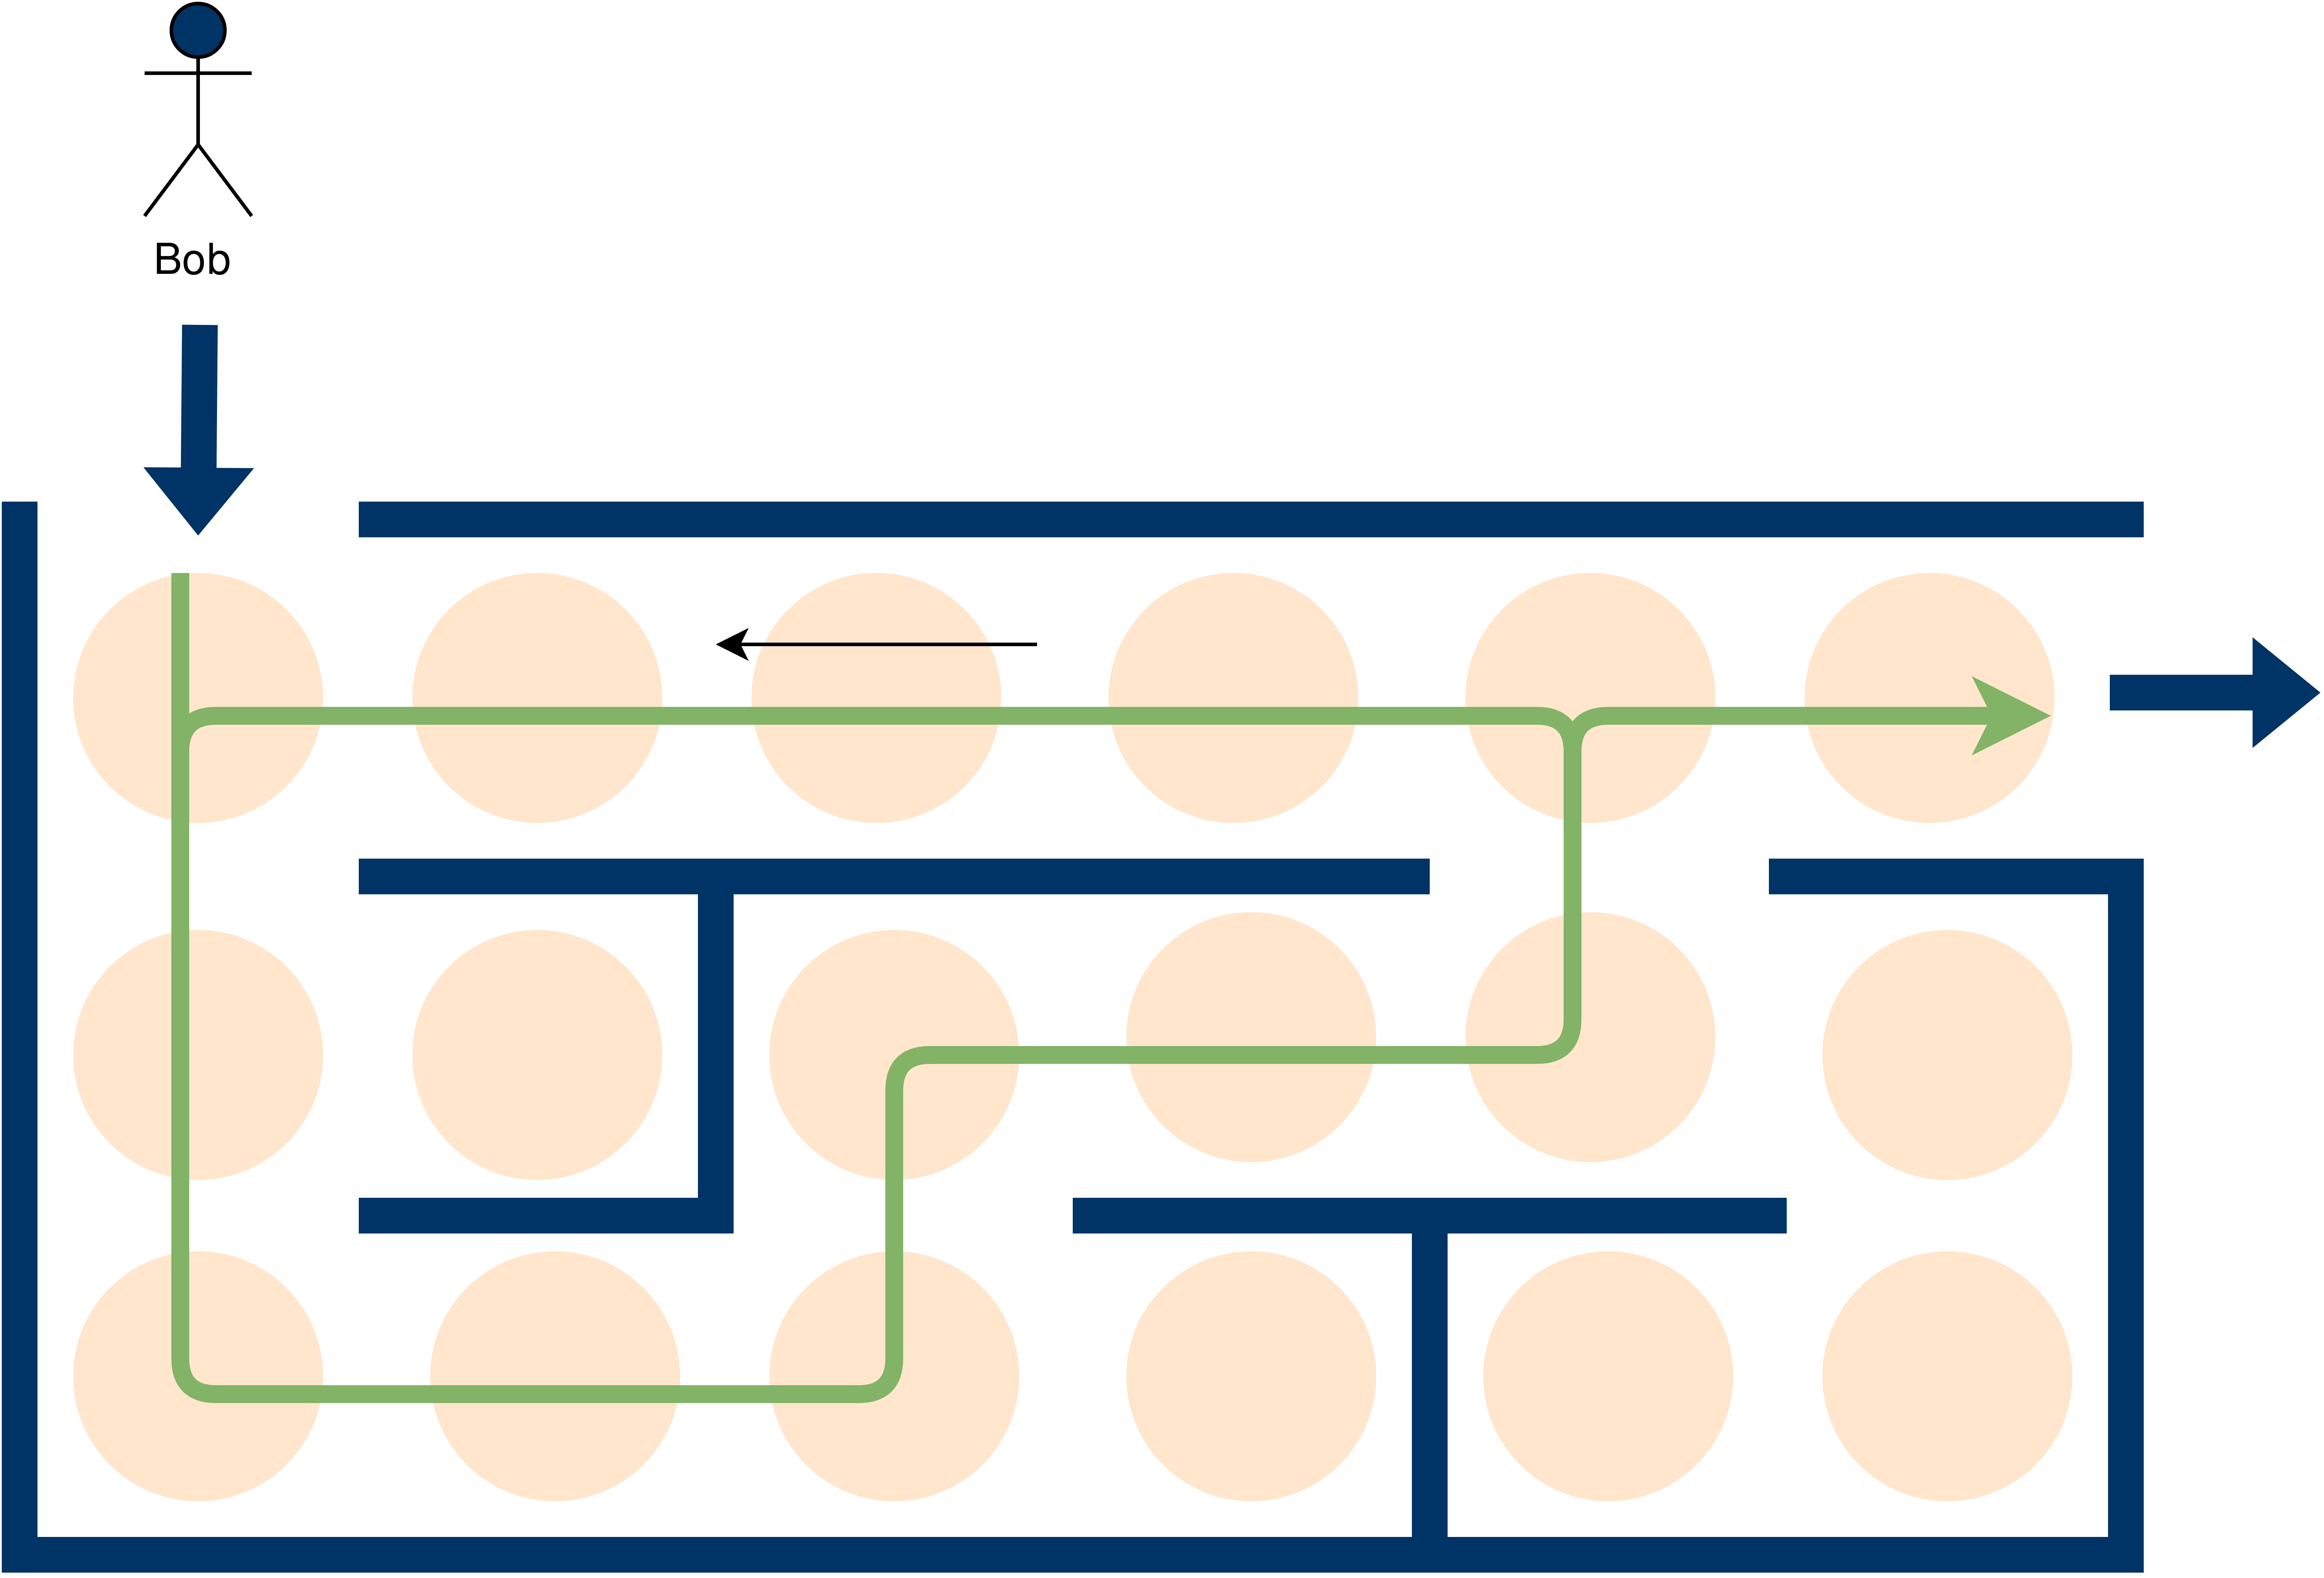
\includegraphics[width=0.7\textwidth]{../figures/GBeispiel4.png}
            \caption{Schlaufe gegen Uhrzeigersinn}

        \end{figure}
    }
\end{frame}
}

{\setbeamercolor{palette primary}{bg=ExColor}
\begin{frame}<handout:0>{Lösung}
    \begin{columns}
        \column{0.45\textwidth}
        \begin{alertblock}{Eine Möglichkeit:}
            %Wir nehmen uns zwei Variablen um zwischen den Einstiegsrichtungen zu unterscheiden für jeden Entscheidungspunkt und konstruieren damit  unsere Grammatik:\\
            $G = (V, \Sigma, P, S)$, wobei \\
            $V = \{S, A_u, A_r, B_u, B_l\}$ \\
            $\Sigma = \{\text{\Rewind}, \text{\MoveUp}, \text{\Forward}, \text{\MoveDown}\}$ \\
            $P = \{S \rightarrow \text\MoveDown A_u \ |\ \text\MoveDown A_r,$\\
            \qquad\; $A_u \rightarrow \text{\Forward\Forward\Forward\Forward} B_l$\\
            \qquad\; $A_r \rightarrow \text{\MoveDown\MoveDown\Forward\Forward\MoveUp\Forward\Forward\MoveUp} B_u,$\\
            \qquad\; $B_l \rightarrow \text{\MoveDown\Rewind\Rewind\MoveDown\Rewind\Rewind\MoveUp\MoveUp} A_u \ |\ \text{\Forward\Forward},$\\
            \qquad\; $B_u \rightarrow \text{\Rewind\Rewind\Rewind\Rewind} A_r \ |\ \text{\Forward\Forward}\}$
        \end{alertblock}
        \column{0.55\textwidth}
        \begin{figure}
            \centering
            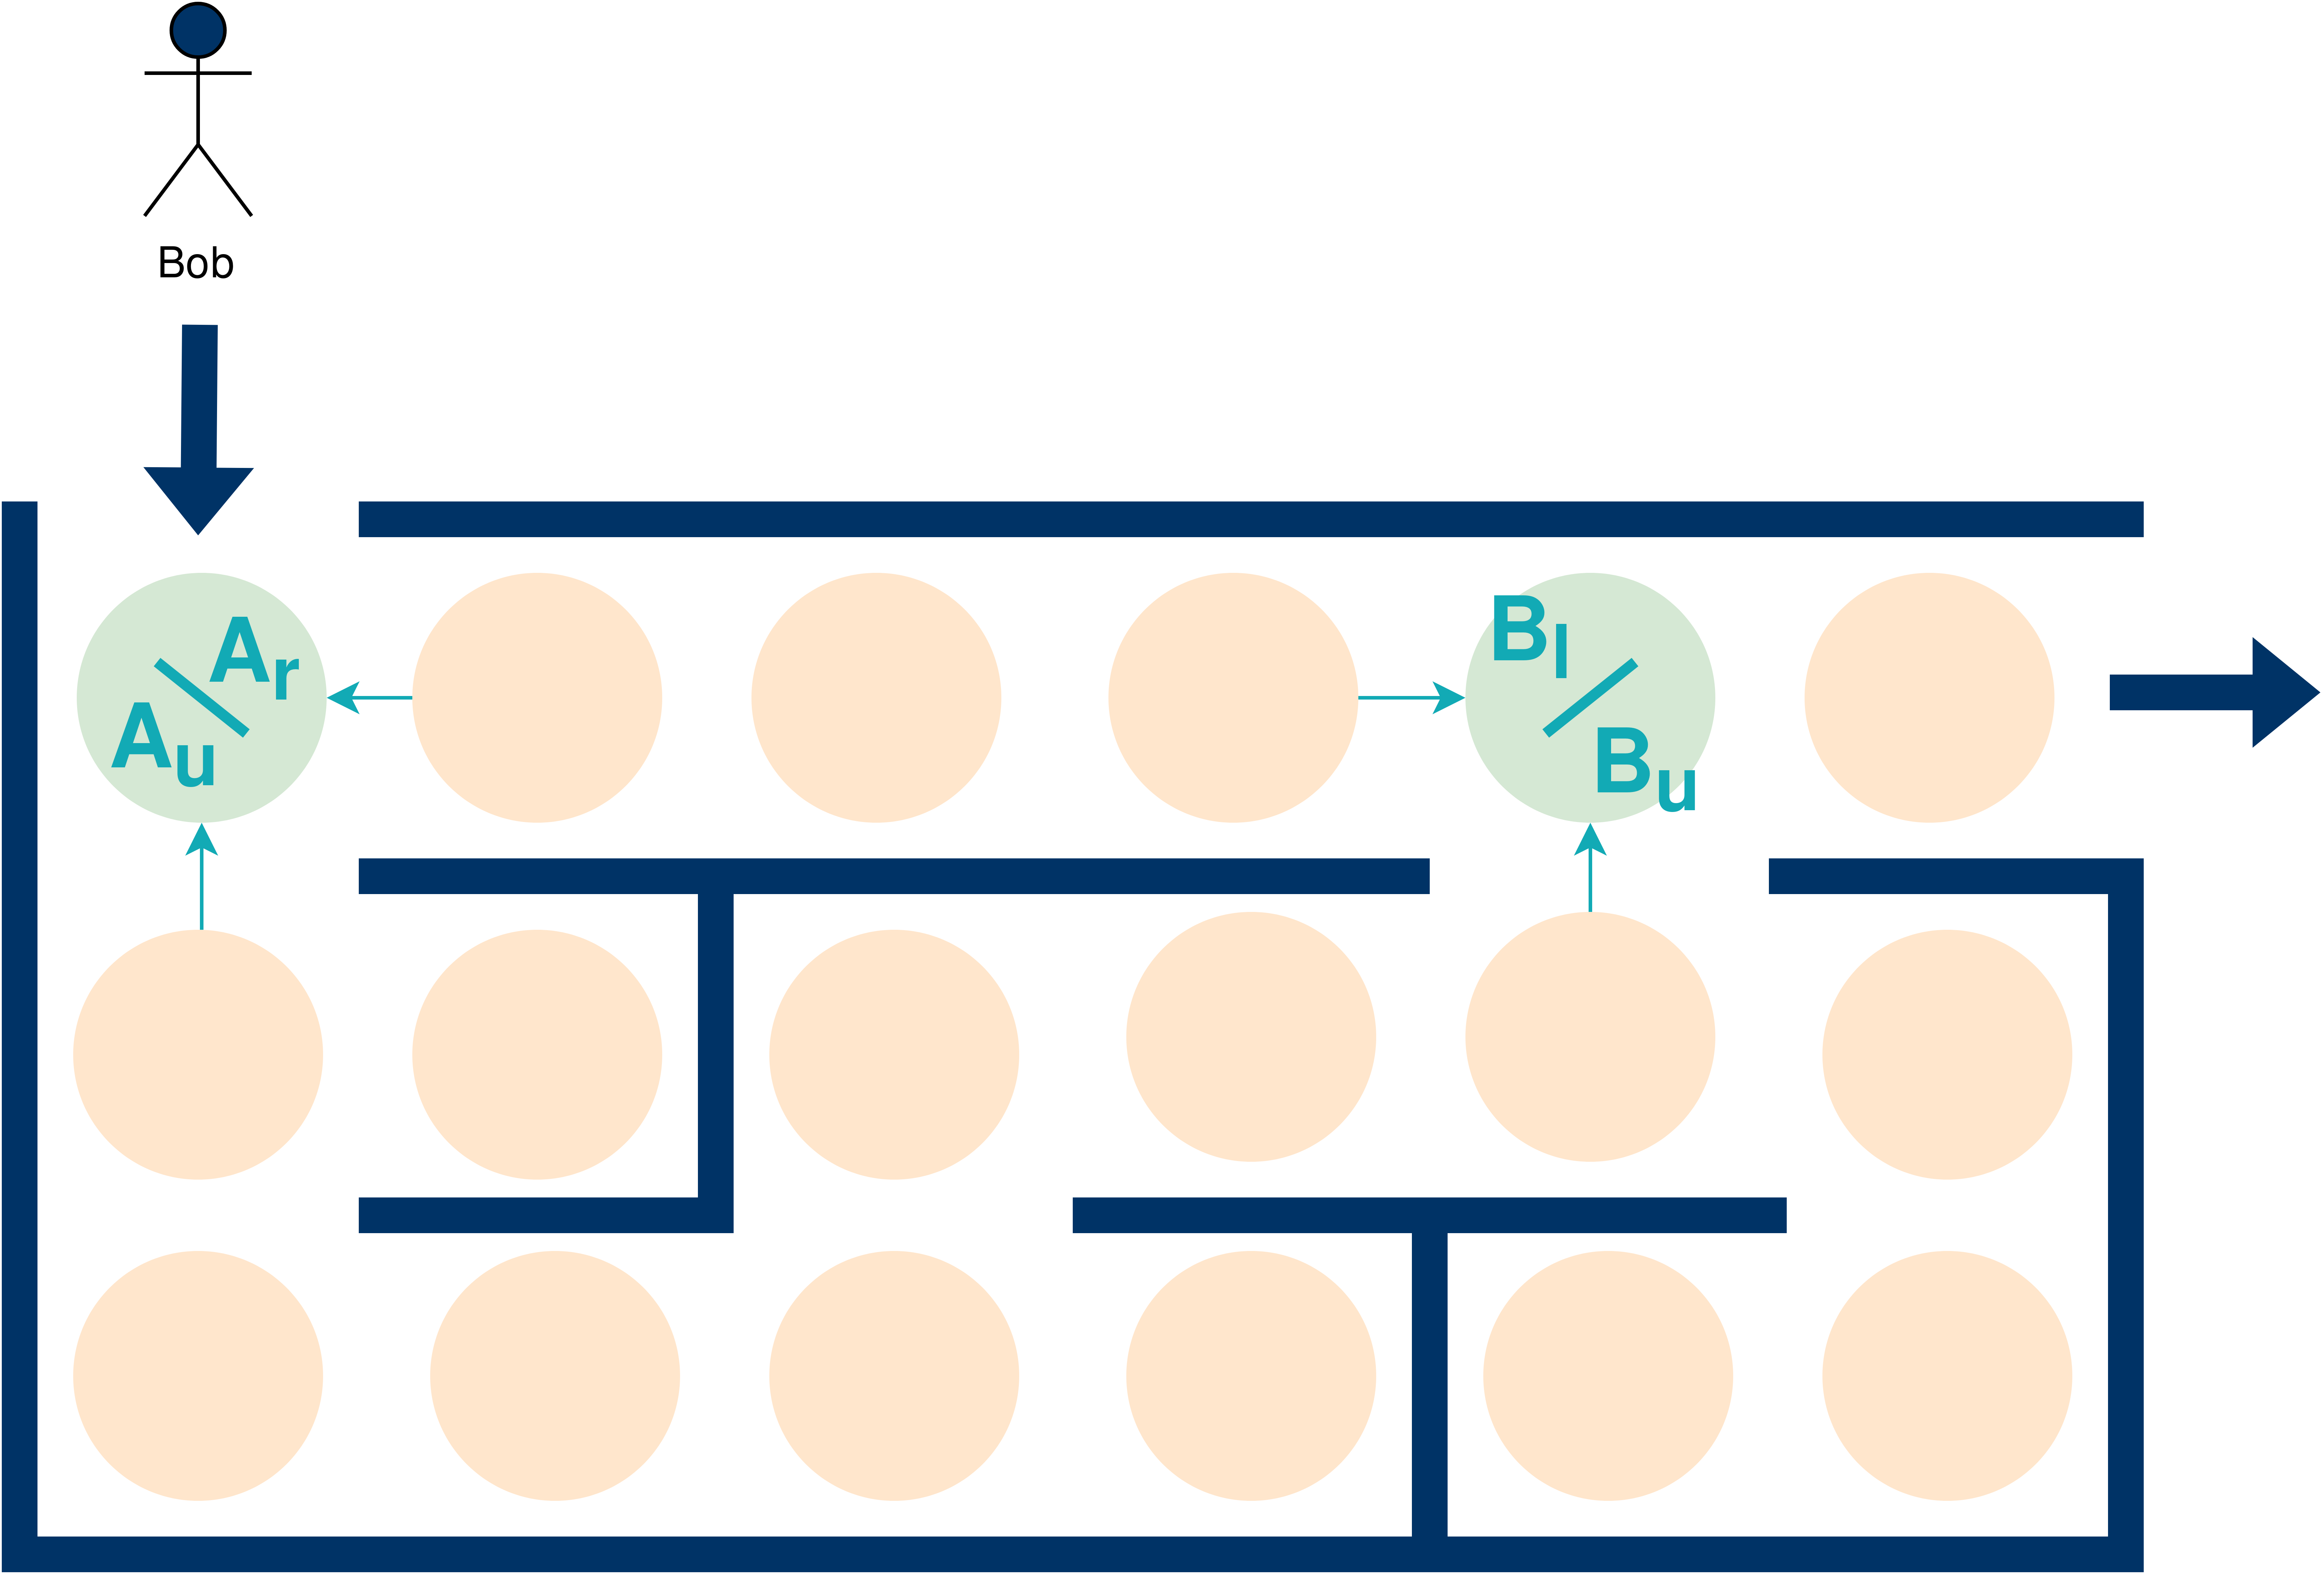
\includegraphics[width=0.9\textwidth]{../figures/GBeispielHowTo.png}
            \caption{Es muss unterschieden werden, ob Bob von links, rechts oder unten kam}

        \end{figure}
    \end{columns}
    \small\emph{Erinnerung:} Bob kann nicht auf ein Feld zurücktreten, von dem er gerade kam
\end{frame}
}

\subsubsection{Ableiten}
\begin{frame}[fragile]{Ableiten}
    Wir können durch das Ableiten formal zeigen, dass ein Wort von einer Grammatik erzeugt wird:\\
    \small{Wir betrachten L = \{$ww^R \mid w^R\text{ ist w rückwärts, }w \in \{a, b\}^n, n\in \mathbb{N}\setminus \{0\}$\}\\
        mit der Grammatik $G=(V,\Sigma,P,S)$, wobei\\
        $V=\{S\}$, $\Sigma=\{a,b\}$, $P = \{S \rightarrow aSa \ |\ bSb \ |\ aa \ |\ bb$\}}
    \metroset{block=fill}
    \begin{exampleblock}{Beispiel}
        Wir zeigen $ww^R = ababbbbaba \in$ L.\\
        \small{$S\Rightarrow_G aSa \Rightarrow_G abSba \Rightarrow_G  abaSaba \Rightarrow_G ababSbaba$ \\ $\Rightarrow_G ababbbbaba$}\\\qed
    \end{exampleblock}
\end{frame}

{\setbeamercolor{palette primary}{bg=ExColor}
\begin{frame}{Denkpause}
    \begin{alertblock}{Aufgaben}
        Zeige die folgenden Aussagen
    \end{alertblock}
    \metroset{block=fill}
    \begin{block}{Normal}
        \begin{itemize}
            \item $P_1=\{S\rightarrow aaS\ |\ \emptyWord\}$ erzeugt $aaaa$
            \item $P_2=\{S\rightarrow AB$, $A\rightarrow aAb \ |\ ab\ |\ \emptyWord$, $B\rightarrow cB \ |\  \emptyWord\}$ erzeugt $aabbc$
            \item $P_3=\{S\rightarrow UV$, $U\rightarrow aU \ |\  bU \ |\  \emptyWord$, $V\rightarrow c \ |\  d\}$ erzeugt $abac$
            \item $P_4=\{S\rightarrow XXX$, $X\rightarrow a \ |\  b \ |\  c\}$ erzeugt $aac$
        \end{itemize}
    \end{block}
    \begin{block}{Etwas Schwerer}
        \begin{itemize}
            \item $P_5=\{S\rightarrow a \ |\  aaaS\}$ erzeugt $aaaa$
            \item $P_6=\{S\rightarrow AAAB$, $AB\rightarrow BA,
                      A\rightarrow cA \ |\  Ac   a,
                      B\rightarrow cB \ |\  Bc \ |\  b\}$ erzeugt $cabcacca$
            \item $P_7=\{S\rightarrow U\text{\Stopsign} \ |\  \text{\Stopsign}$, $U\rightarrow \text{\Rewind} U \ |\  \text{\MoveUp} U \ |\  \text{\Forward} U \ |\  \text{\MoveDown} U \ |\ \emptyWord\}$ erzeugt \Forward\Stopsign
        \end{itemize}
    \end{block}
\end{frame}
}

{\setbeamercolor{palette primary}{bg=ExColor}
\begin{frame}<handout:0>{Lösungen}
    Alle Lösungen sind Beispiellösungen, es sind auch andere möglich.
    \begin{itemize}[<+- | alert@+>]
        \item $S\Rightarrow_G aaS \Rightarrow_G aaaaS \Rightarrow_G aaaa$
        \item $S\Rightarrow_G AB \Rightarrow_G aAbB \Rightarrow_G aabbB \Rightarrow_G aabbcB \Rightarrow_G aabbc$
        \item $S\Rightarrow_G UV \Rightarrow_G aUV \Rightarrow_G abUV \Rightarrow_G abaUV \Rightarrow_G abaV \Rightarrow_G abac$
        \item $S\Rightarrow_G XXX \Rightarrow_G aXX \Rightarrow_G aaX \Rightarrow_G aac$
        \item $S\Rightarrow_G aaaS \Rightarrow_G aaaa$
        \item $S\Rightarrow_G AAAB \Rightarrow_G AABA \Rightarrow_G ABAA \Rightarrow_G cABAA \Rightarrow_G caBAA \Rightarrow_G cabAA \Rightarrow_G cabcAA \Rightarrow_G cabcaA\Rightarrow_G cabcacA \Rightarrow_G cabcaccA \Rightarrow_G cabcacca$
        \item $S\Rightarrow_G U\text{\Stopsign} \Rightarrow_G \text{\Forward}U\text{\Stopsign} \Rightarrow_G \text{\Forward}\text{\Stopsign}$
    \end{itemize}
\end{frame}
}
